% ### Erste Seite der Grenzschichten ###
\centering
\vspace{31mm} %44mm
\section*{\myul{Grenzschichten}}

\begin{tikzpicture}[remember picture, overlay]

% --- ERSTE REIHE: Am Seitenursprung anfangen
\setlength{\rowheight}{22mm}

    % A1) Erste Kachel relativ zum Seitenursprung
    \setlength{\cellwidth}{46mm}
    \Tile{A1}{([xshift=10mm, yshift=-68mm]current page.north west)}{\cellwidth}{\rowheight}
        {
            \vspace{-\TileSep}
            \titlebf{Wandschubspannung}\\ \vspace{-2mm}
            \begin{equation*}
                \tau_0 = \frac{\rho\,v_\infty^2}{6}\,\frac{\text{d}\delta}{\text{d}x}
            \end{equation*}
        }{0}{1}{1}{0}

    % B1) Zweite Kachel rechts anbauen
    \setlength{\cellwidth}{46mm}
    \Tile{B1}{(A1.north east)}{\cellwidth}{\rowheight}
        {
            \vspace{-\TileSep}
            \titlebf{Grenzschichtdicke}\\ \vspace{-2mm}
            \begin{equation*}
                \frac{\delta}{x} = \sqrt{\frac{12\,\nu}{v_\infty\,x}} = \sqrt{\frac{12}{\mathrm{Re}_x}}
            \end{equation*}
        }{0}{1}{1}{0}

    % C1) Dritte Kachel rechts anbauen
    \setlength{\cellwidth}{98mm}
    \Tile{C1}{(B1.north east)}{\cellwidth}{\rowheight}
        {
            \vspace{-\TileSep}
            \titlebf{Widerstandsbeiwert}\\ \vspace{1mm}
            \begin{minipage}[t]{0.48\cellwidth-\TileSep}
                \centering
                \titlerm{Lokal}\\ \vspace{-4mm}
                \begin{equation*}
                    c_\text{f} = \frac{2}{\sqrt{12\,\mathrm{Re}_x}} = \frac{2\,\tau_0(x)}{\rho\,v_\infty^2}
                \end{equation*}
            \end{minipage}%
            \vline
            \begin{minipage}[t]{0.52\cellwidth-\TileSep}
                \centering
                \titlerm{Gesamt}\\ \vspace{-4mm}
                \begin{equation*}
                    c_\text{W} = 2\,\sqrt{\frac{\nu}{3\,v_\infty\,x}} = \frac{2}{\sqrt{3\,\mathrm{Re}_x}}
                \end{equation*}%
                \vspace{-2.25mm}
            \end{minipage}
        }{0}{0}{1}{0}

% --- ZWEITE REIHE: Unten anbauen
\setlength{\rowheight}{15mm}

    % X2) Eigene Zeile für die Überschrift
    \Tile{X2}{(A1.south west)}{190mm}{8mm}
        {
            \titlebf{Grenzschichtgleichungen}
        }{0}{0}{0}{0}

    % A2) Erste Kachel unten anbauen
    \setlength{\cellwidth}{50mm}
    \Tile{A2}{(X2.south west)}{\cellwidth}{\rowheight}
        {
            \vspace{-\TileSep}
            \titlerm{Kontinuitätsgleichung}\\ \vspace{-4mm}
            \begin{equation*}
                \frac{\partial u}{\partial x} + \frac{\partial v}{\partial y} = 0
            \end{equation*}
        }{0}{1}{1}{0}

    % B2) Zweite Kachel rechts anbauen
    \setlength{\cellwidth}{28mm}
    \Tile{B2}{(A2.north east)}{\cellwidth}{\rowheight}
        {
            \vspace{-\TileSep}
            \titlerm{$y$-Impuls}\\ \vspace{-4mm}
            \begin{equation*}
                \frac{\partial p}{\partial y} = 0
            \end{equation*}
        }{0}{1}{1}{0}

    % C2) Dritte Kachel rechts anbauen
    \setlength{\cellwidth}{58mm}
    \Tile{C2}{(B2.north east)}{\cellwidth}{\rowheight}
        {
            \vspace{-\TileSep}
            \titlerm{$x$-Impuls}\\ \vspace{-4mm}
            \begin{equation*}
                u\,\frac{\partial u}{\partial x} + v\,\frac{\partial u}{\partial y} = -\frac{1}{\rho}\,\frac{\partial p}{\partial x} + \nu\,\frac{\partial^2 u}{\partial y^2}
            \end{equation*}
        }{0}{1}{1}{0}

    % D2) Vierte Kachel rechts anbauen
    \setlength{\cellwidth}{54mm}
    \Tile{D2}{(C2.north east)}{\cellwidth}{\rowheight}
        {
            \vspace{-\TileSep}
            \titlerm{Randbedingungen}\\ \vspace{-5mm}
            \begin{equation*}
                \underbrace{u = v = 0}_{y\,=\,0}\qquad \underbrace{u = u_\delta(x)}_{y\,=\,\delta}
            \end{equation*}
        }{0}{0}{1}{0}

% --- DRITTE REIHE: Unten anbauen
\setlength{\rowheight}{17mm}

    % X3) Eigene Zeile für die Überschrift
    \Tile{X3}{(A2.south west)}{190mm}{8mm}
        {
            \titlebf{Blasius-Gleichung}
        }{0}{0}{0}{0}

    % A3) Erste Kachel unten anbauen
    \setlength{\cellwidth}{32mm}
    \Tile{A3}{(X3.south west)}{\cellwidth}{\rowheight}
        {
            \vspace{-\TileSep}
            \titlerm{Variable}\\ \vspace{-3.25mm}
            \begin{equation*}
                \eta = y\,\sqrt{\frac{v_\infty}{\nu\,x}} = \frac{y}{\delta}
            \end{equation*}
        }{0}{1}{1}{0}

    % B3) Zweite Kachel rechts anbauen
    \setlength{\cellwidth}{40mm}
    \Tile{B3}{(A3.north east)}{\cellwidth}{\rowheight}
        {
            \vspace{-\TileSep}
            \titlerm{Stromfunktion}\\ \vspace{-2.5mm}
            \begin{equation*}
                \Psi(x,y) = \sqrt{v_\infty\,\nu\,x}\cdot f\!\left(\eta\right)
            \end{equation*}
        }{0}{1}{1}{0}

    % C3) Dritte Kachel rechts anbauen
    \setlength{\cellwidth}{36mm}
    \Tile{C3}{(B3.north east)}{\cellwidth}{\rowheight}
        {
            \vspace{-\TileSep}
            \titlerm{Blasius-Gleichung}\\ \vspace{-3mm}
            \begin{equation*}
                f''' + \frac{1}{2}\,f\,f'' = 0
            \end{equation*}
        }{0}{1}{1}{0}

    % D3) Vierte Kachel rechts anbauen
    \setlength{\cellwidth}{82mm}
    \Tile{D3}{(C3.north east)}{\cellwidth}{\rowheight}
        {
            \vspace{-\TileSep}
            \titlerm{Randbedingungen}\\ \vspace{1mm}
            \begin{minipage}[t]{0.5\cellwidth-\TileSep}
                \centering
                \myul{$y = 0$ / $\eta = 0$:}\\ \vspace{-5mm}
                \begin{equation*}
                    u = v = f(0) = f'(0) = 0
                \end{equation*}
            \end{minipage}%
            \vline
            \begin{minipage}[t]{0.5\cellwidth-\TileSep}
                \centering
                \myul{$y\rightarrow\infty$ / $\eta\rightarrow\infty$:}\\ \vspace{-5mm}
                \begin{equation*}
                    u = v_\infty~~\vline~~f'(\eta\ll 1) = 1
                \end{equation*}%
                \vspace{-4.75mm}
            \end{minipage}
        }{0}{0}{1}{0}

% --- VIERTE REIHE: Unten anbauen
\setlength{\rowheight}{120mm}

    % A4) Erste Kachel unten anbauen
    \setlength{\cellwidth}{60mm}
    \Tile{A4}{(A3.south west)}{\cellwidth}{\rowheight}
        {
            \titlerm{Lösungen}\\ \vspace{2mm}
            \begin{tabular}{c|c|c|c}
                \xrowht[()]{2.8mm} \cellcolor{Gray!40}$\eta$ & \cellcolor{Gray!40}$f$ & \cellcolor{Gray!40}$f'$ & \cellcolor{Gray!40}$f''$ \\ \hline
                \xrowht[()]{2.8mm} 0   & 0      & 0      & 0,3321 \\ \hline
                \xrowht[()]{2.8mm} 0,5 & 0,0415 & 0,1659 & 0,3309 \\ \hline
                \xrowht[()]{2.8mm} 1,0 & 0,1656 & 0,3298 & 0,3230 \\ \hline
                \xrowht[()]{2.8mm} 1,5 & 0,3701 & 0,4868 & 0,3026 \\ \hline
                \xrowht[()]{2.8mm} 2,0 & 0,6500 & 0,6298 & 0,2668 \\ \hline
                \xrowht[()]{2.8mm} 2,5 & 0,9963 & 0,7513 & 0,2174 \\ \hline
                \xrowht[()]{2.8mm} 3,0 & 1,3968 & 0,8460 & 0,1614 \\ \hline
                \xrowht[()]{2.8mm} 3,5 & 1,8377 & 0,9130 & 0,1078 \\ \hline
                \xrowht[()]{2.8mm} 4,0 & 2,3057 & 0,9555 & 0,0642 \\ \hline
                \xrowht[()]{2.8mm} 4,5 & 2,7901 & 0,9795 & 0,0340 \\ \hline
                \xrowht[()]{2.8mm} 5,0 & 3,2833 & 0,9915 & 0,0159 \\ \hline
                \xrowht[()]{2.8mm} 5,5 & 3,7806 & 0,9969 & 0,0066 \\ \hline
                \xrowht[()]{2.8mm} 6,0 & 4,2796 & 0,9990 & 0,0024 \\ \hline
                \xrowht[()]{2.8mm} 6,5 & 4,7793 & 0,9997 & 0,0008 \\ \hline
                \xrowht[()]{2.8mm} 7,0 & 5,2792 & 0,9999 & 0,0002 \\ \hline
                \xrowht[()]{2.8mm} 7,5 & 5,7792 & 1,0000 & 0,0001 \\ \hline
                \xrowht[()]{2.8mm} 8,0 & 6,2792 & 1,0000 & 0,0000
            \end{tabular}
        }{0}{1}{0}{0}

    % B4) Erste Kachel unten anbauen
    \setlength{\cellwidth}{130mm}
    \Tile{B4}{(A4.north east)}{\cellwidth}{\rowheight}
        {
            \titlerm{Ebene Platte (Laminar)}\\ \vspace{2mm}
            \begin{minipage}[t]{0.3\cellwidth-\TileSep}
                \centering
                \titlerm{Wandschubspannung}\\ \vspace{-3mm}
                \begin{equation*}
                    \tau_0 = \frac{\text{0,3321}\,\rho\,v_\infty^2}{\sqrt{\mathrm{Re}_x}}
                \end{equation*}
            \end{minipage}%
            \vline
            \begin{minipage}[t]{0.4\cellwidth-\TileSep}
                \centering
                \titlerm{Lokaler Widerstandsbeiwert}\\ \vspace{-3mm}
                \begin{equation*}
                    c_f = \frac{\text{0,6642}}{\sqrt{\mathrm{Re}_x}}\quad\vline\quad c_\text{W} = \frac{\text{1,328}}{\sqrt{\mathrm{Re}_x}}
                \end{equation*}
            \end{minipage}%
            \vline
            \begin{minipage}[t]{0.3\cellwidth-\TileSep}
                \centering
                \titlerm{Grenzschichtdicke}\\ \vspace{-3mm}
                \begin{equation*}
                    \delta = \frac{5\,x}{\sqrt{\mathrm{Re}_x}} \sim x^{\text{0,5}}
                \end{equation*}
            \end{minipage}%
            \vspace{1.75mm} \rule{\dimexpr\cellwidth-2\TileSep}{0.5pt} \\ \vspace{0.5mm}
            \titlerm{Keil}\\ \vspace{1mm}
            \begin{minipage}[t]{0.3\cellwidth-\TileSep}
                \centering
                \vspace{-24mm}
                \begin{equation*}
                    m = \frac{\theta}{2\,\pi - \theta}
                \end{equation*}%
                \vspace{-1mm}
                \begin{equation*}
                    u_\delta \approx x^m
                \end{equation*}
            \end{minipage}%
            \begin{minipage}[t]{0.5\cellwidth-\TileSep}
                \centering
                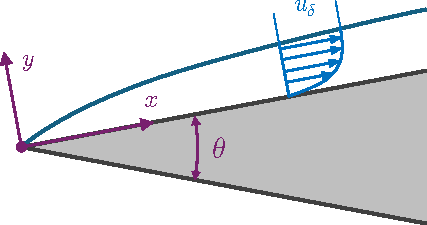
\includegraphics[width=0.4\cellwidth]{images/keil.pdf}
            \end{minipage}
            \vspace{1mm} \rule{\dimexpr\cellwidth-2\TileSep}{0.5pt} \\ \vspace{1.5mm}
            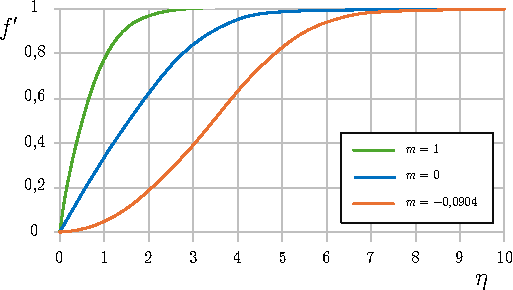
\includegraphics[width=0.6\cellwidth]{images/blasius-gleichung-graph.pdf}
            \begin{minipage}{0.45\cellwidth-\TileSep}
                \centering
                \scriptsize
                \begin{align*}
                    m = 1&:~\text{Ebene Staupunktströmung} \\
                    m = 0&:~\text{Ebene Platte}
                \end{align*}
            \end{minipage}%
            \begin{minipage}{0.45\cellwidth-\TileSep}
                \centering
                \scriptsize
                \begin{align*}
                    m = \text{-0,0904}&:~\text{Grenzfall} \\
                    m < \text{-0,0904}&:~\text{Strömungsablösung}
                \end{align*}
            \end{minipage}
        }{0}{0}{0}{0}

\end{tikzpicture}